% the pdf attachments are generated with 
% - visualize.ipynb within ./SVM/

\documentclass[oneside]{ctexbook}
\usepackage{graphicx} % Required for inserting images
\usepackage{amsmath}
\usepackage{amssymb}
\usepackage{amsthm}
\usepackage[unicode]{hyperref}
\usepackage{geometry}
\geometry{a4paper, left=1in, right=1in, top=1in, bottom=1in}
\usepackage{minted}

\usepackage{enumitem}
\setlist[itemize]{noitemsep}
\setlist[enumerate]{noitemsep} % remove item separation for all lists
\usepackage{titling}
\title{《人工智能与机器学习基础》第三次实验报告}
\author{PB24000150 李欣宸}

\date{\today}

\begin{document}

\renewcommand{\maketitlehookd}{\begin{center}报告为了保持简短，没有包含数学推导过程。所有数学推导详见我的博客：

    \href{https://xinchengo.github.io/blog-zh/2025/12/23/支持向量机决策树与集成学习/}{\tt https://xinchengo.github.io/blog-zh/2025/12/23/支持向量机决策树与集成学习/}

    该博客是我在完成作业三和实验三的过程中同步编写的
    \end{center}}

\maketitle

\tableofcontents

\chapter{支持向量机实验}

\section{实验原理}

\subsection{HTRU2 数据集}

作为“中国物理大学”的学生，我们有理由弄清楚本实验使用的 \href{https://archive.ics.uci.edu/dataset/372/htru2}{HTRU2 数据集}是什么。

脉冲星一般由射电望远镜探测得到，“中国天眼”就是射电望远镜中的一个典型。截至 2024 年 11 月，“天眼”已经发现超过 1000 颗脉冲星，典型的检测流程是这样的：

\begin{itemize}
    \item 先假定不同的{\bf 色散量}（Dispersion Measure, DM），对收集到的信号进行色散矫正；
    
    脉冲星发出的信号包含很广的波段，由于宇宙空间中有很多等离子体，这些波段在到达地球的过程中会发生色散现象；矫正后我们才能得到其真正的光度曲线；

    当假定的色散量与真实色散量相同的时候，信噪比最高；假定色散量和去色散后信噪比之间的曲线，我们称为{\bf 色散量-信噪比曲线}（Dispersion Measure--Signal to Noise Ratio Curve, DM-SNR curve）；

    \item 综合脉冲星多个周期的信号，得到{\bf 积分脉冲轮廓}（Integrated Pulse Profile），注意它不是 \ref{fig:rotating-pulsar} 的光度曲线；积分轮廓的均值、标准差对应其“亮度”作为总体得到的统计量。
\end{itemize}

DM-SNR 曲线和积分脉冲轮廓都能反映脉冲星的性质：真实的脉冲星 DM-SNR 曲线应符合某种性质（用物理方法得到）；积分脉冲轮廓在亮度极低处有一个较为明显的峰（峰度系数大，极度左偏，偏度系数大），因为脉冲星光度大的时刻非常短暂。

数据集包括：

\begin{itemize}
    \item 积分轮廓的均值、标准差、峰度系数（kurtosis）、偏度系数（skewness）；
    \item DM-SNR 曲线的均值、标准差、峰度系数、偏度系数；
\end{itemize}

\begin{figure}[htbp]
    \centering
    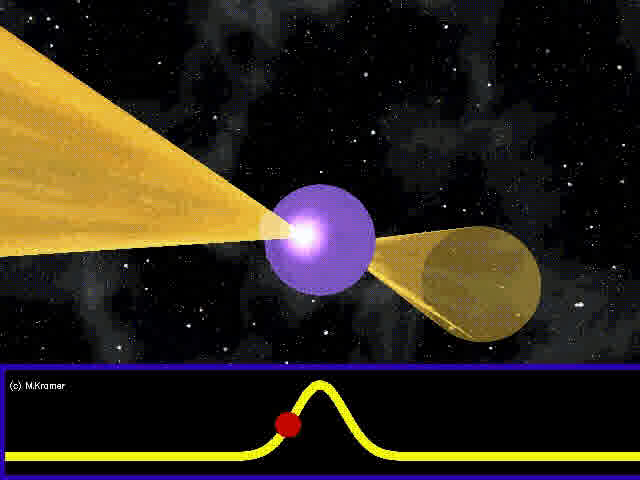
\includegraphics[width=0.3\textwidth]{assets/pulsar.jpg}
    \label{fig:rotating-pulsar}
    \caption{脉冲星光度曲线的形成}
    （来源：维基百科）
\end{figure}

\subsection{支持向量机}

可以参考\href{https://xinchengo.github.io/blog-zh/2025/12/23/%E6%94%AF%E6%8C%81%E5%90%91%E9%87%8F%E6%9C%BA%E5%86%B3%E7%AD%96%E6%A0%91%E4%B8%8E%E9%9B%86%E6%88%90%E5%AD%A6%E4%B9%A0/#%E6%94%AF%E6%8C%81%E5%90%91%E9%87%8F%E6%9C%BA}{我的博客中“支持向量机”部分}的内容。本篇报告中{\bf 不包含}数学推导过程，所有推导均在博客中给出。

\section{代码补全情况说明}

补全了 \verb|submission.py| 中挖空的地方，并解决了一处错误（）；书写了 \verb|visualize.ipynb| 以绘制部分图表；修改了 \verb|visualization.py| 中关于热力图的细节。

\section{实验结果和分析}

\subsection{数据集可视化}

加载 \verb|pulsar.csv| 可以使用 Pandas 库；观察到数据集中有较多（25.98\%）的样本在某些特征上存在缺失值（NaN）。题目附带的 \verb|dataloader.py| 中已经包含了用中位数填充缺失值的代码。

我的可视化代码见 \verb|visualize.ipynb|。

\subsubsection{特征的分布和相关性}

研究特征分布时对每个特征忽略了 NaN 值（我们猜想其真实值分布与正常值相近）。

\begin{figure}[htbp]
    \centering
    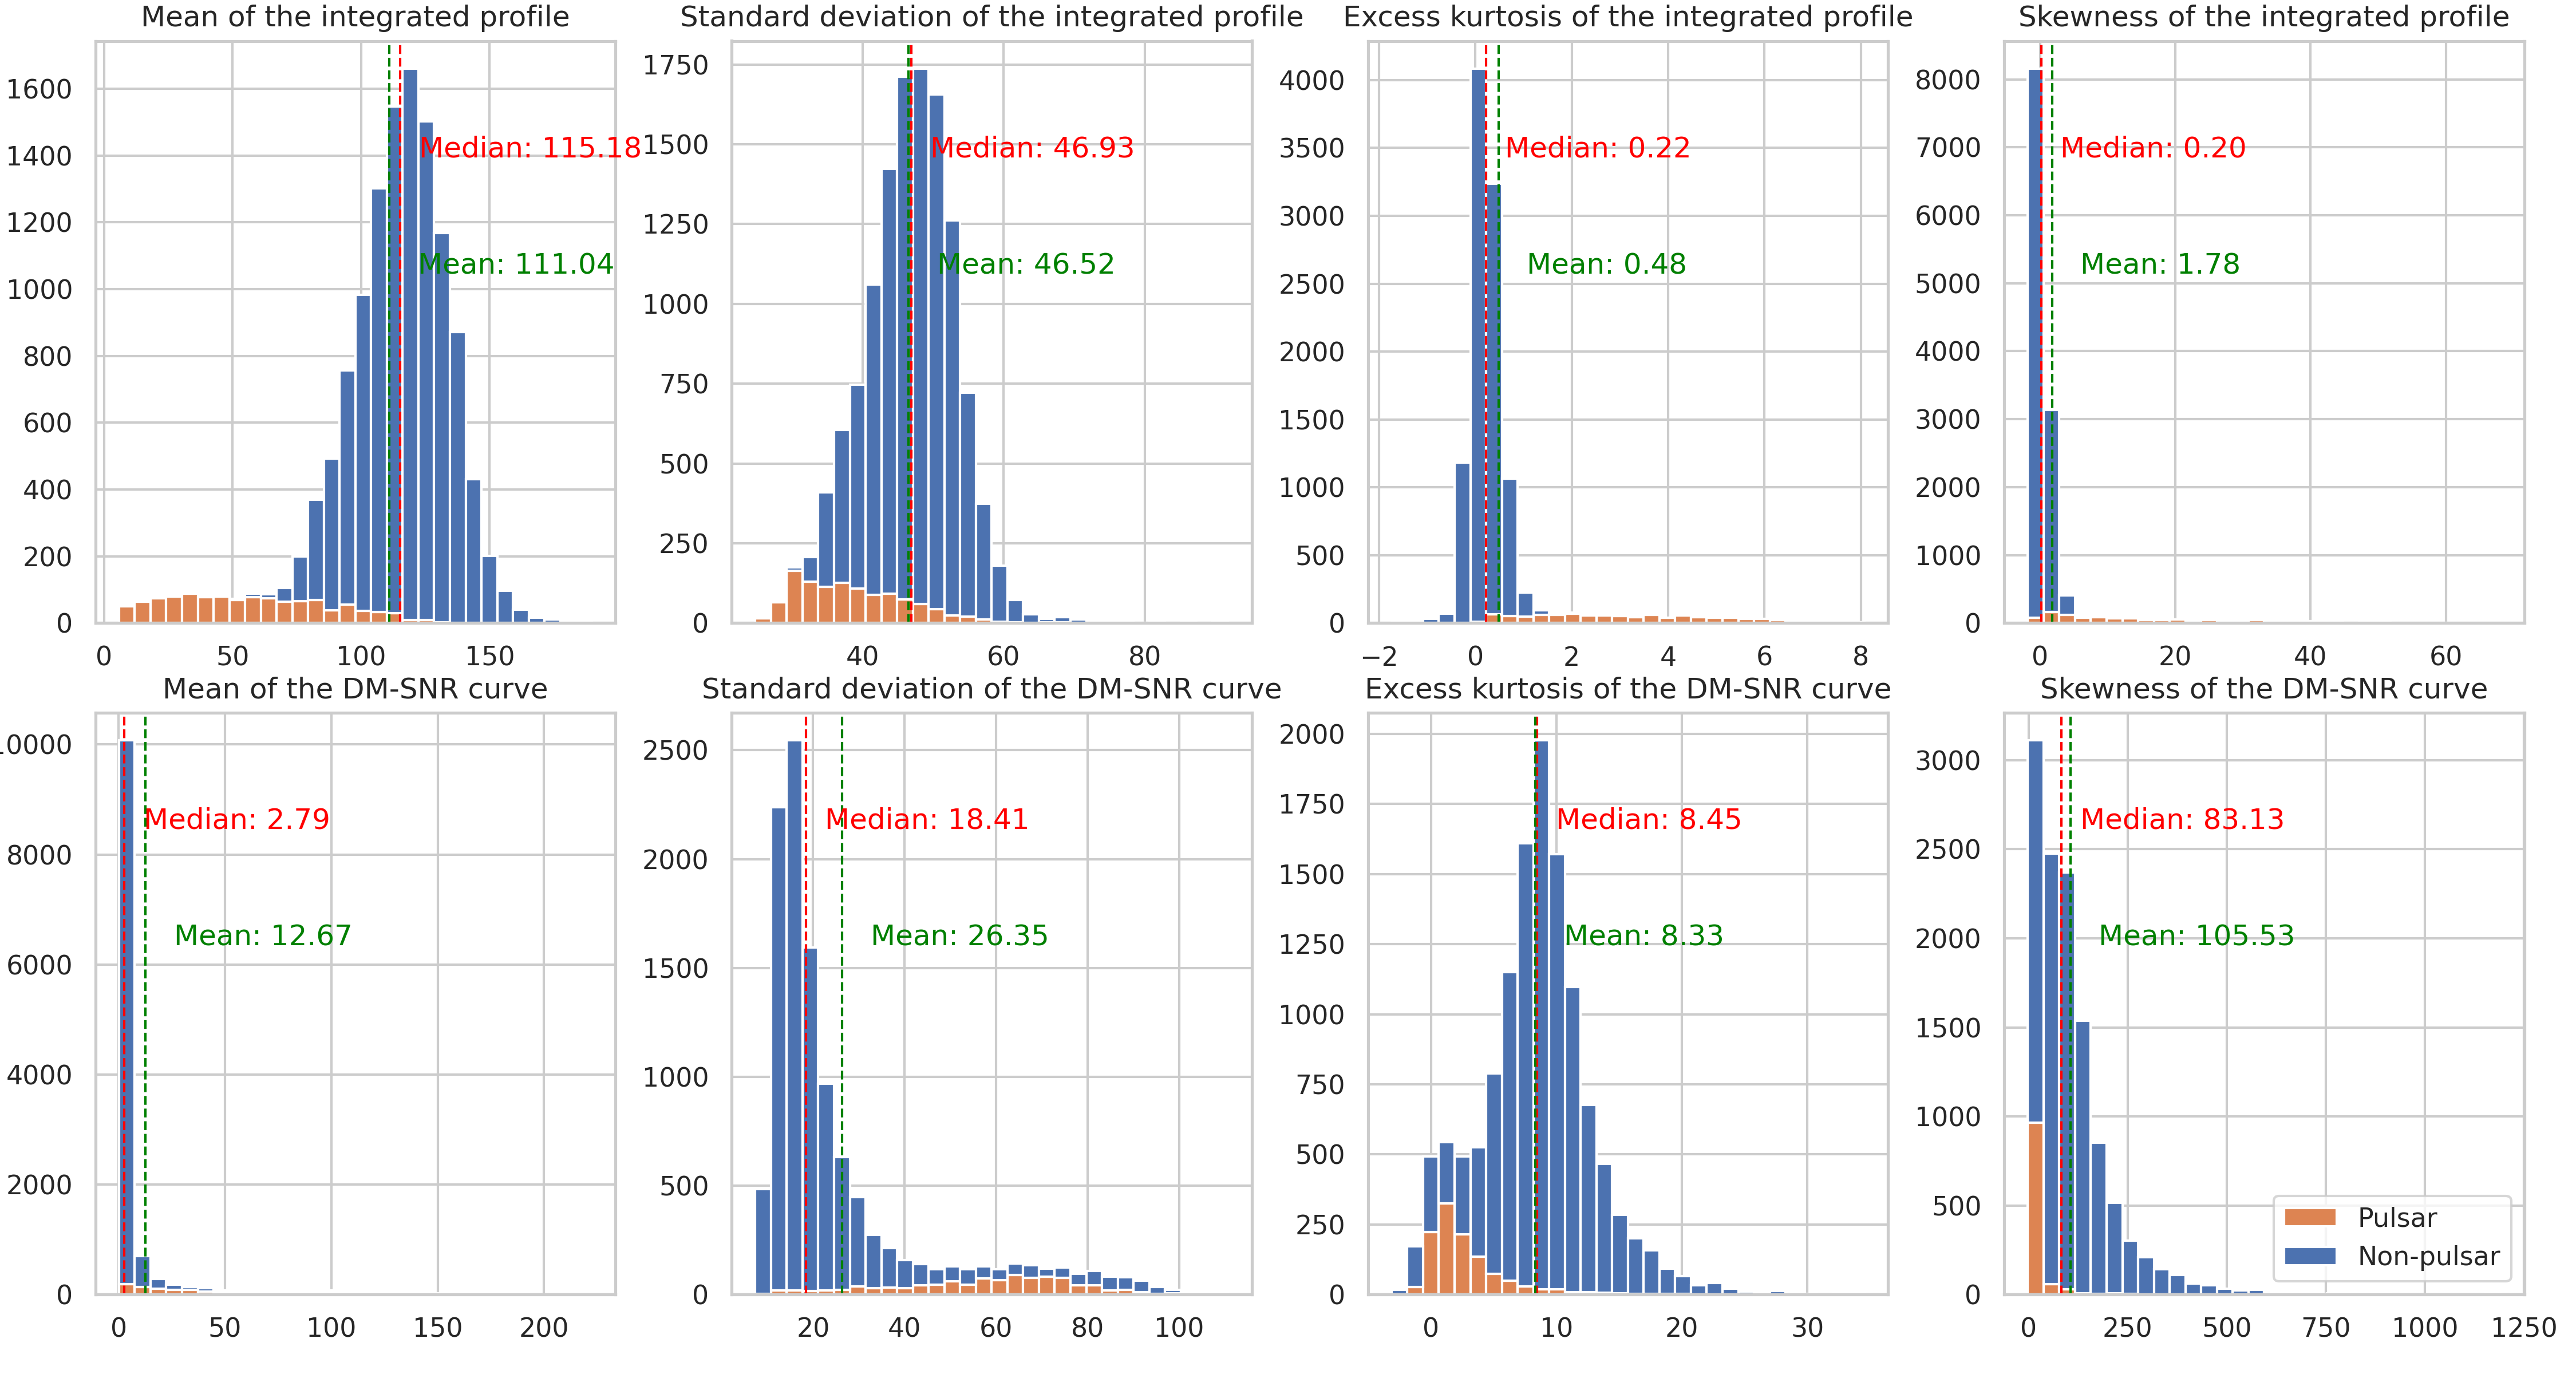
\includegraphics[width=1.0\textwidth]{assets/feature_distributions.pdf}
    \vspace{-3em}
    \caption{各特征的分布直方图}
    \label{fig:feature-distributions}
\end{figure}

\begin{figure}[t]
    \centering
    \includegraphics[width=0.8\textwidth]{assets/correlation_heatmap.pdf}
    \vspace{-1.5em}
    \caption{各特征的相关性热力图}
    \label{fig:correlation-heatmap}
\end{figure}

图 \ref{fig:correlation-heatmap} 可以看到，所有特征可以比较好地划分为两组（第一组积分轮廓的均值标准差和 DM-SNR 曲线的峰度偏度，第二组其他），组内成正相关，组间成负相关；第一组与结果大致呈负相关，第二组与结果大致呈正相关。其中以两组峰度、偏度系数间的相关性最为显著。

与分类相关性最大的特征是积分轮廓的峰度系数（79\%）、积分轮廓的偏度系数（71\%）、积分曲线的均值（-68\%）；这三点都由真实脉冲星积分轮廓极度左偏的形状决定。

\subsubsection{PCA 降维}

PCA 使用了 \verb|feature_engineering.py| 中的 \verb|PCAProjector|。

\begin{figure}[t]
    \centering
    \includegraphics[width=0.6\textwidth]{assets/pca_scatter.pdf}
    \vspace{-1.5em}
    \caption{PCA 降维后前两主成分的散点图}
    \label{fig:pca-scatter}
\end{figure}

可以看出，降维后的负样本形如一个高斯椭球，正样本分布形如椭圆但没有明显中心。前两维度可以较好地区分绝大多数正负样本。

\subsection{线性核 SVM 的可视化} \label{sec:linear-svm-visualization}

本节探讨超参数 $C$ 对软间隔 SVM 决策的影响。由于样本太多（见 \ref{para:about-dataset-quality}），难以直观感受，因此本届的可视化实验都是用随机抽取的 500 个样本进行的。

\begin{figure}[htbp]
    \centering
    \includegraphics[width=0.99\textwidth]{assets/svm_all_kernel_decision_boundaries.pdf}
    \vspace{-1.5em}
    \caption{不同 C 值下三种核 SVM 的决策边界}
    \label{fig:svm-all-kernel-decision-boundaries}
\end{figure}

由 \ref{fig:svm-all-kernel-decision-boundaries} 可见，随着 $C$ 值增大，间隔和支持向量数目均减小。

这其实可以从软间隔 SVM 的目标函数 \eqref{eq:soft-margin-svm} 理解：

\begin{equation}
\begin{matrix}
\displaystyle \min_{w,b,\zeta} & \displaystyle \frac{1}{2}\|w\|^2+C\sum_{i=1}^n\zeta_i^2 \\
\text{s.t.} &  y_i(w^Tx_i+b)\ge 1 - \zeta_i,~\zeta_i \ge 0
\end{matrix}
\label{eq:soft-margin-svm}
\end{equation}

$C$ 越大，模型能“容忍”的误分类越少，支持向量越少，其决策边界越受少量局部向量的影响。若数据中有较多噪声点，$C$ 过大会导致过拟合；比如上图中 $C=10^6$ 时，F1 分数略有下降；对比 $C=5$ 时，红、蓝色的支持向量涵盖整个红、蓝交界的区域，$C=10^6$ 时，支持向量集中在红、蓝交界中心处。

\subsection{非线性核 SVM 的可视化} \label{sec:nonlinear-svm-visualization}

本节探讨核函数类型和超参数 $d$（多项式核）$\gamma$（RBF 核）对 SVM 决策的影响。如图结论：

\begin{itemize}
    \item  $d\nearrow~\implies$ 决策边界复杂性 $\nearrow,~\mathrm{\#NS}\searrow$（见图 \ref{fig:svm-all-kernel-decision-boundaries}）； 
    \item $\gamma \nearrow~\implies$ 决策边界复杂性 $\nearrow,~\mathrm{\#NS}\searrow$（见图 \ref{fig:svm-all-kernel-decision-boundaries}）。
    \item 此外，当多项式核度数为偶数和奇数时，决策边界形状也有明显差异。
\end{itemize}

这是因为 $d$ 控制多项式核对应特征空间中多项式的次数，次数越高，模型越复杂；而 $\gamma$ 控制特征空间中，系数随次数和距离增加的衰减速率，$\gamma$ 越大，高次项对内积的贡献越大，模型越复杂。具体的数学解释见\href{https://xinchengo.github.io/blog-zh/2025/12/23/%E6%94%AF%E6%8C%81%E5%90%91%E9%87%8F%E6%9C%BA%E5%86%B3%E7%AD%96%E6%A0%91%E4%B8%8E%E9%9B%86%E6%88%90%E5%AD%A6%E4%B9%A0/#%E6%A0%B8%E5%87%BD%E6%95%B0%E4%B8%8E%E6%A0%B8%E6%8A%80%E5%B7%A7}{我的博客}。

\subsection{超参数调优可视化} \label{sec:hyperparameter-tuning-visualization}

我对 RBF 核 SVM 使用网格搜索（Grid Search）调优超参数 $C$ 和 $\gamma$，\ref{fig:grid_heatmap} 为 F1 分数热力图。可以看到，$C$ 的增大和 $\gamma$ 增大对模型起到的作用是相反的：$C$ 增大对模型复杂度起到约束作用，而 $\gamma$ 减少降低了高次项对内积的贡献，也降低模型复杂度。

表现最优的点大致集中在一条直线上，我猜测是 $C$ 和 $\gamma$ 之间的相互作用造成的。

\begin{figure}[htbp]
    \centering
    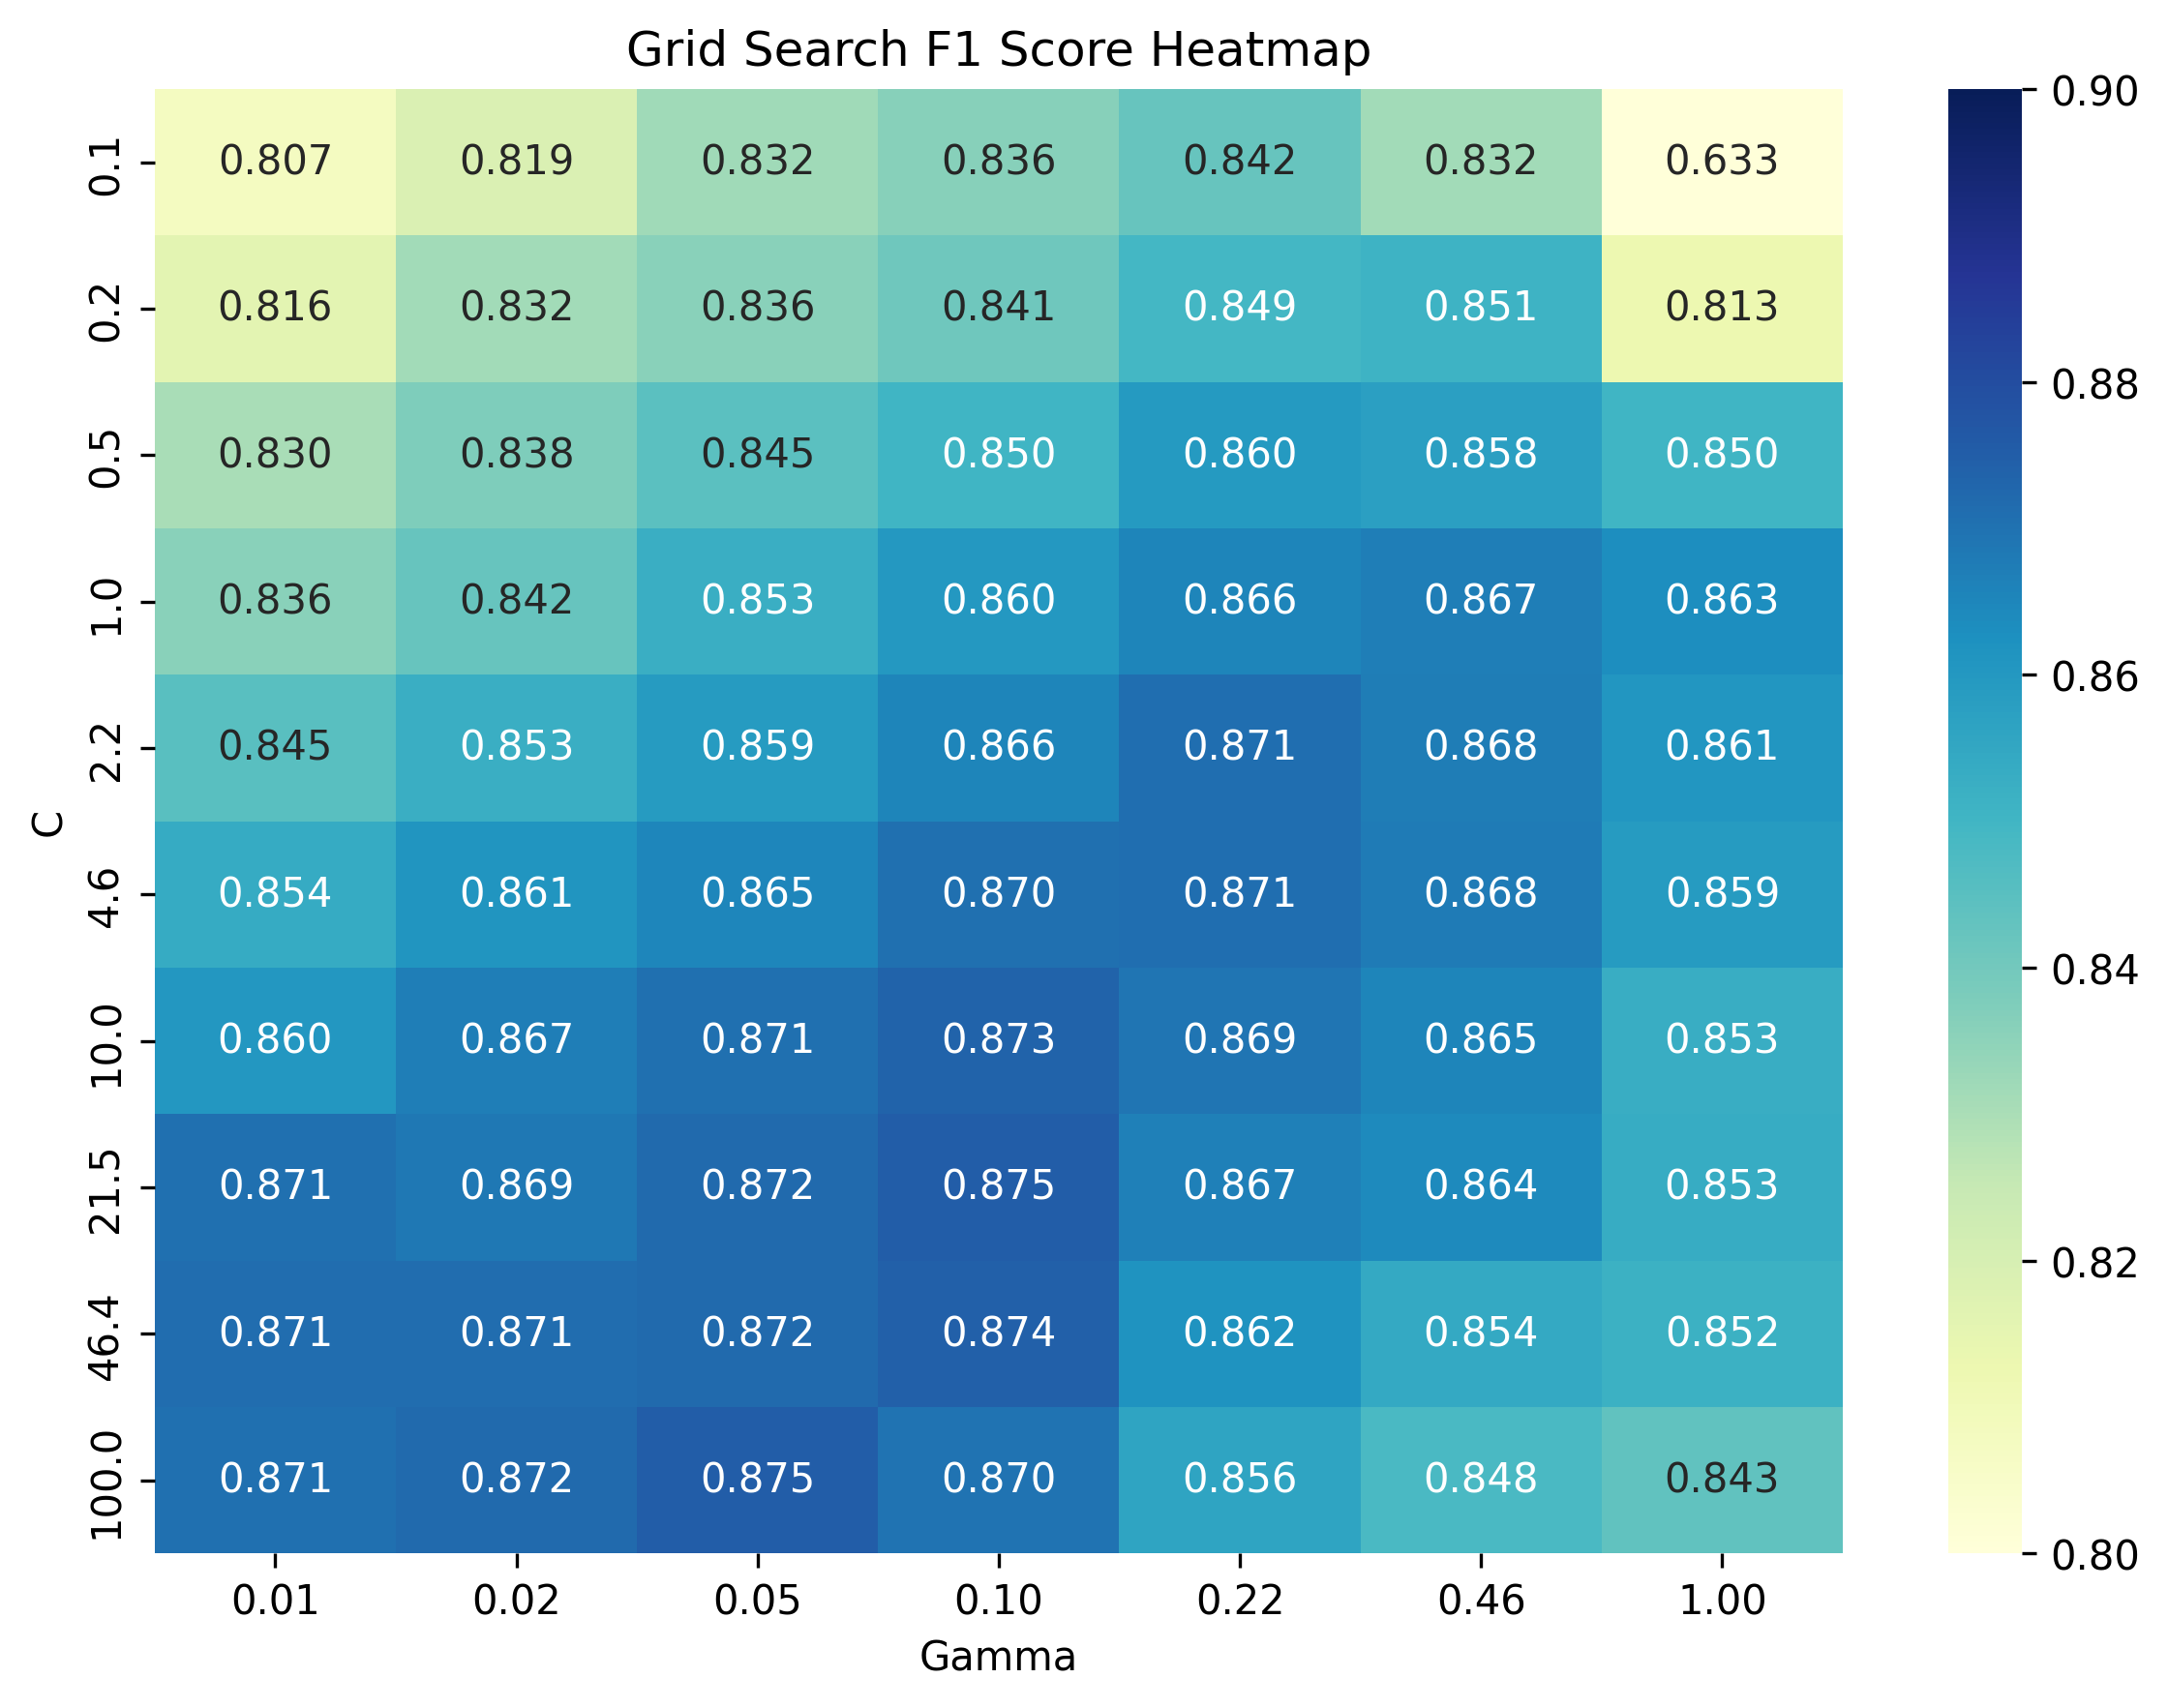
\includegraphics[width=0.7\textwidth]{assets/grid_heatmap_f1.png}
    \vspace{-1.5em}
    \caption{RBF 核 SVM 超参数调优热力图}
    \label{fig:grid_heatmap}
\end{figure}

\section{思考题回答}

\subsubsection{为什么 SVM 要最大化间隔？} 

考虑对训练数据“加噪”，最大化间隔可以最大化模型对“噪声”的容错性；如果我们考虑稍微“移动”一下决策边界，那么最大化间隔等同于最大化若要改变分类，决策边界需要移动的距离；注意上面这段分析有意义的前提是特征空间的“距离”有意义，以及噪声服从高斯假设。

\subsubsection{C 越大越容易过拟合，为什么？}

从直观的角度理解（也可参考 \ref{sec:linear-svm-visualization}）：
\begin{gather*}
    C \nearrow \implies \text{（由 \eqref{eq:soft-margin-svm}）对误分类的容忍度} \searrow \implies \mathrm{\#NS} \searrow \\
    \implies \text{决策边界更受少量局部向量影响} \nearrow \implies \text{过拟合风险} \nearrow
\end{gather*}

\subsubsection{RBF 核中的 $\gamma$ 太大有什么问题}

RBF 核的特征空间是无限维的，$\gamma$ 控制了高次项对内积的贡献；当 $\gamma$ 趋于无穷大时，模型的表示能力趋于无限强，直到把整个训练集都过拟合（如 \ref{fig:svm-all-kernel-decision-boundaries} 中 $\gamma=1$ 的情形）。

\subsubsection{为什么支持向量数少，模型更容易泛化？}


这个命题其实并{\bf 不}总是成立，应当从两方面看待：
\begin{itemize}
    \item 一般模型复杂度 $\searrow \implies$ 支持向量数 $\searrow$，而较为简单的模型往往更容易泛化；
    \item 但是对于同一类模型，当我们调整 $C\nearrow$，支持向量数 $\searrow$ 可能使模型更容易受到少量极端样本的影响，从而导致过拟合，泛化能力下降。
\end{itemize}

\subsubsection{Polynomial 核的 degree 越大有什么影响？}

\href{https://xinchengo.github.io/blog-zh/2025/12/23/%E6%94%AF%E6%8C%81%E5%90%91%E9%87%8F%E6%9C%BA%E5%86%B3%E7%AD%96%E6%A0%91%E4%B8%8E%E9%9B%86%E6%88%90%E5%AD%A6%E4%B9%A0/#%E6%A0%B8%E5%87%BD%E6%95%B0%E4%B8%8E%E6%A0%B8%E6%8A%80%E5%B7%A7}{由数学解释}，degree 越大，模型的表示能力越强，决策边界越复杂；但是可以通过增加常数项 $c$ 来控制模型复杂度。

\section{思考与难点}

\subsection{困惑与思考}

\paragraph{关于“写好报告”的梦想与实践中的挫折}

在听完郑悟强助教对实验一的讲解后我心潮澎湃，感受到这门课“写报告”的实际意义是培养我们的科学思维（实事求是，写好做每一步的原因，而不是盲目堆砌结果），所以我非常希望能把本次报告写好。

可视化决策边界的过程是实验最精华的部分。但是按照报告要求画出各类图表的过程让我觉得有些繁琐；\verb|visualization.py| 中的代码有少量错误且不能涵盖所有画图需求，要真的花好图需要自己写一个 Jupyter NoteBook。

\paragraph{代码错误} \verb|submission.py| 有错，\verb|KernelSVM| 的 \verb|KernelManager| 应在 \verb|fit| 中声明而不是在 \verb|__init__| 中声明；因为 \verb|GridSearchCV| 中只会创建一个 \verb|KernelSVM| 实例，改变参数使用的是 \verb|BaseEstimator| 中的 \verb|set_params| 方法；\verb|KernelManager| 只会被初始化一次，导致不同核函数的 SVM 都使用了同一个核函数。

\subsection{对实验的建议}

\paragraph{关于数据集质量} \label{para:about-dataset-quality}

实验中使用的 HTRU2 数据集是原始 \href{https://archive.ics.uci.edu/dataset/372/htru2}{HRU2 数据集}的一个 70\% 大小的一个子集，但是令人不解的是，数据集中有很多缺失值（25.98\% 的行存在 NaN 项），而原始 HRU2 数据集中就没有。

数据规模太大，高度线性可分，导致超参数提升、核函数选择等对结果影响不大。而 SVM 主要优势在于处理小规模、高维度的数据集。

\chapter{决策树实验}

\section{代码补全情况说明}

补全了 \verb|decision_tree.ipynb| 中挖空的地方。

\section{实验经过}

该节主要讲述我补全 \verb|decision_tree.ipynb| 的简要结果以及我对决策树原理的简要介绍。

\subsection{原理}

决策树，顾名思义是对决策过程的树形建模：每个结点按照一个相对简单的标准将数据分成两组或多组；以此形成递归的决策结构；

常用的决策树算法往往会做以下的妥协：

\begin{itemize}
    \item 每个结点（也被称为 Decision Stump）只对一个特征进行分类——这样得到的决策树具有更强的{\bf 可解释性}；斜决策树（oblique decision tree）放宽了这一限制；
    \item 贪心构造，对每个结点，优先选择本次分裂后最优化某种{\bf 分类判据}的特征；这样就避免了最优决策树（Optimal Decision Tree, ODT）的求解（它是 NP-完全的）；比如 ID3 算法就以熵增最大化（entropy gain）作为分裂判据；
\end{itemize}

更多的介绍在此处省略，可以参考\href{https://xinchengo.github.io/blog-zh/2025/12/23/%E6%94%AF%E6%8C%81%E5%90%91%E9%87%8F%E6%9C%BA%E5%86%B3%E7%AD%96%E6%A0%91%E4%B8%8E%E9%9B%86%E6%88%90%E5%AD%A6%E4%B9%A0/#%E5%86%B3%E7%AD%96%E6%A0%91}{我的博客中“决策树”部分的章节}。

\subsection{实验结果}

补全实验代码的过程较为顺利。实验代码的实现中稍微复习了 \verb|numpy| 一些基本操作的运用。

得到的结果完美区分了 10 项数据，最后一个单元格的输出如下所示：

\begin{verbatim}
     Depth 0, Root: Split on feature: 2
    - Depth 1, Left: Split on feature: 0
      -- Left leaf node with indices [0, 1, 4, 7]
      -- Right leaf node with indices [5]
    - Depth 1, Right: Split on feature: 1
      -- Left leaf node with indices [8]
      -- Right leaf node with indices [2, 3, 6, 9]
\end{verbatim}

\chapter{集成学习实验}

\section{代码补全情况说明}

补全了 \verb|submission.py| 中挖空的地方（包括拓展实验）；书写了 \verb|visualize.ipynb| 以绘制部分图表；修改了 \verb|visualization.py| 的部细节；在 \verb|train.py| 添加了随机种子设置。

\verb|create_fig.sh| 是用于生成实验所需图表的自动化脚本。

\section{实验原理}

我在\href{https://xinchengo.github.io/blog-zh/2025/12/23/%E6%94%AF%E6%8C%81%E5%90%91%E9%87%8F%E6%9C%BA%E5%86%B3%E7%AD%96%E6%A0%91%E4%B8%8E%E9%9B%86%E6%88%90%E5%AD%A6%E4%B9%A0/#%E9%9B%86%E6%88%90%E5%AD%A6%E4%B9%A0}{博客}中书写了一部分数学公式的推导，可作参考。

\section{实验结果和分析}

\subsection{混淆矩阵} \label{sec:confusion-matrix}

图 \ref{fig:confusion-matrix} 展示了五种集成学习方法在测试集上的混淆矩阵。

\begin{figure}[hb]
    \centering
    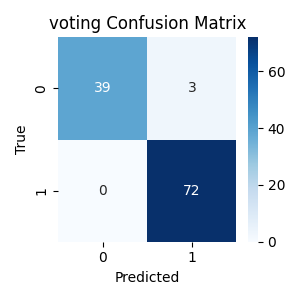
\includegraphics[width=0.32\textwidth]{assets/voting_cm.png}
    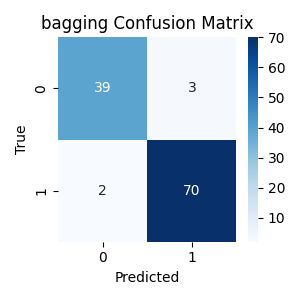
\includegraphics[width=0.32\textwidth]{assets/bagging_cm.png}
    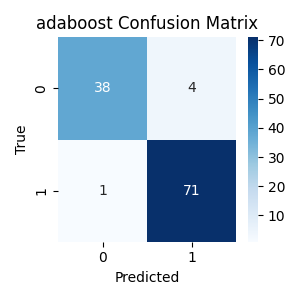
\includegraphics[width=0.32\textwidth]{assets/adaboost_cm.png}
    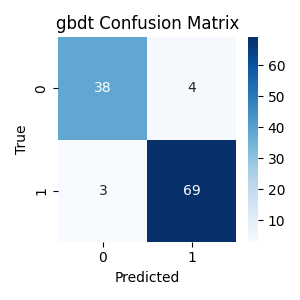
\includegraphics[width=0.32\textwidth]{assets/gbdt_cm.png}
    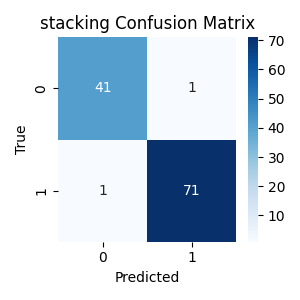
\includegraphics[width=0.32\textwidth]{assets/stacking_cm.png}
    \vspace{-1.5em}
    \caption{五种集成学习方法的混淆矩阵}
    \label{fig:confusion-matrix}
\end{figure}

通过混淆矩阵可以得到各方法的准确率和 F1 分数，见表 \ref{tab:overall-performance}。

\begin{table}[t]
    \centering
    \begin{tabular}{lcc}
        \hline
        方法 & 准确率 & F1 分数 \\
        \hline
        Voting & 0.9737 & 0.9735 \\
        Bagging & 0.9561 & 0.9560 \\
        AdaBoost & 0.9561 & 0.9558 \\
        GBDT & 0.9386 & 0.9384 \\
        Stacking & 0.9825 & 0.9825 \\
        \hline
    \end{tabular}
    \caption{三种集成学习方法的整体性能对比}
    \label{tab:overall-performance}
\end{table}

\subsection{AdaBoost 的效果与弱学习器数量的关系}

图 \ref{fig:adaboost-training-error} 展示了 AdaBoost 在训练集上的误差下降曲线。

\begin{figure}[t]
    \centering
    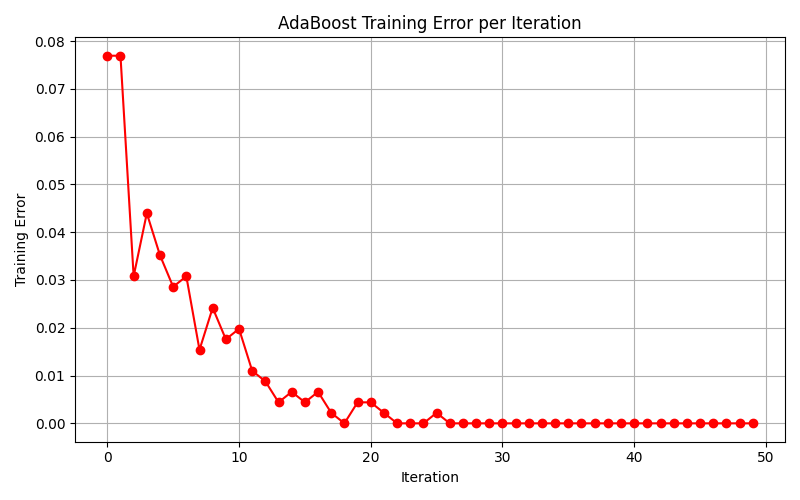
\includegraphics[width=0.7\textwidth]{assets/adaboost_training_curve.png}
    \vspace{-1.5em}
    \caption{AdaBoost 的训练误差下降曲线}
    \label{fig:adaboost-training-error}
\end{figure}

训练误差随着弱学习器数量的增长快速下降到 0（26 个弱学习器时），我们猜测模型发生了过拟合，下面我们使用{\it 交叉验证}（绝对不能用测试集）和{\it 可视化决策边界}两种方法进行验证，结果显示没有发生明显的过拟合。

\subsubsection{交叉验证的结果}

我使用 5 折交叉验证评估了不同弱学习器数量下 AdaBoost 的表现，指标选取验证集上的准确率和 F1 分数（图 \ref{fig:adaboost-cv-performance}），随着学习器数量的增加，模型表现虽略有波动，但总体较为稳定，没有发生明显的过拟合。这与课上“AdaBoost 对过拟合有较强的稳健性”结论一致。

\subsubsection{可视化决策边界}

可以看到，学习器数量增加后，决策边界仍然简单，清晰，没有明显过拟合的迹象（图 \ref{fig:adaboost-decision-boundaries}）。


\subsection{简化版 GBDT 的性质}

本实验中使用的简化版 GBDT 用学习率取代了线搜索，其性能不如 AdaBoost（见表 \ref{tab:overall-performance}）；决策边界可视化表明决策边界复杂性受学习率影响很大（图 \ref{fig:gbdt-decision-boundaries}）：

\begin{figure}[htbp]
    \centering
    \includegraphics[width=0.48\textwidth]{assets/adaboost_cv_accuracy.pdf}
    \includegraphics[width=0.48\textwidth]{assets/gbdt_cv_loss.pdf}
    \vspace{-1.5em}
    \caption{不同弱学习器数量下 AdaBoost 和 GBDT 的交叉验证表现}
    \label{fig:adaboost-cv-performance}
\end{figure}

\begin{figure}[htbp]
    \centering
    \includegraphics[width=0.8\textwidth]{assets/adaboost_decision_boundaries.pdf}
    \vspace{-1.5em}
    \caption{不同弱学习器数量下 AdaBoost 的决策边界}
    \label{fig:adaboost-decision-boundaries}
\end{figure}

\begin{figure}[htbp]
    \centering
    \includegraphics[width=0.8\textwidth]{assets/gbdt_decision_boundaries.pdf}
    \vspace{-1.5em}
    \caption{不同学习率下 GBDT 的决策边界}
    \label{fig:gbdt-decision-boundaries}
\end{figure}

\begin{itemize}
    \item 学习率较大时，决策边界变得曲折；但是模型没有发生过拟合（见图 \ref{fig:adaboost-cv-performance}）；这是因为较大的学习率让每次迭代的“步子”变大，容易出现“矫枉过正”的现象。
    \item 两种学习率下，模型都是欠拟合；
\end{itemize}

可视化中使用的所有 GBDT 中弱学习器均采取最大深度为 1 的决策树（Decision Stump）。



\begin{figure}
    
\end{figure}




\subsection{整体性能的对比}

见 \ref{sec:confusion-matrix}。$\text{Voting} > \text{AdaBoost} > \text{Bagging}$，但是由于数据集线性可分性较强，而且没有对模型参数量进行控制，该结果意义有限。

\section{思考题回答}

\subsection{简答题}

\subsubsection{Voting 和 Bagging 在模型融合机制上的本质区别}

其本质区别在于，Voting 中所有模型都是在相同的训练数据上训练的，而 Bagging（Boostrap Aggregating，自助聚集）算法中，模型是在经过{\bf 自助采样}的数据集上训练的。

\subsubsection{AdaBoost 能用弱分类器构建强分类器的原因}

\begin{equation}
    \alpha_{i,t+1} = \alpha_{i,t}\exp\left( -y_i\hat{w}_tf_t(x_i) \right)
    = \begin{cases}
        \alpha_{i, t} e^{\hat{w}_t} & y_i = f_t(x_i) \\
        \alpha_{i, t} e^{-\hat{w}_t} & y_i \ne f_t(x_i) \\
    \end{cases}
    \label{eq:adaboost-weight-update}
\end{equation}

\paragraph{直观理解}由 \eqref{eq:adaboost-weight-update}，AdaBoost 在每次训练过后提高了错误样本的权重，降低正确样本的权重。这样使得后续的分类器能够有针对性地“弥补”之前分类器的“错误”，从而逐渐拟合一个复杂的数据集。

\paragraph{非线性}众所周知，线性函数的线性组合仍然是线性函数，AdaBoost 的非线性来源于弱分类器的非线性（Decision Stump 是二值函数）。

\subsubsection{Bagging 降低方差，Boosting 降低偏差的理解}

该题为 HW3 的原题。

Bagging（自助聚集）法降低方差的来源是其对数据集进行的再采样（自助采样）；自助采样可以“模拟”真实数据采样过程中随机性造成的影响，如果训练得到的模型相互独立，那么模型的方差会以 $\mathcal O(n^{-1})$ 的速率下降。

而 Boosting 算法的核心是用简单、小的分类器的组合去拟合复杂的函数关系；所以，它达成的目的是降低偏差。

\subsection{选做实验的思考题}

\subsubsection{Gradient Boosting 的优势}

AdaBoost 是 Gradient Boosting 中使用指数损失的特殊形式；所以要分析 GBDT 相较于 AdaBoost 的优势需要从损失函数入手，对比：

\begin{itemize}
    \item AdaBoost 中的指数损失：$\ell (y, F) = e^{-yF}$；
    \item 本题中我们使用的交叉熵损失：$\ell (y, F) = \log(1 + e^{-yF})$；
\end{itemize}

交叉熵损失相比指数损失更加“平缓”，相比指数损失，对噪声的容忍度更高，因此在训练步数较少时能有更“好”的决策边界。但是本实验中{\bf 简化版}的 GBDT 和真正（使用线搜索）的 GBDT 是有很大差别的，所以实验结果难以很好反映两者的差异。

\subsubsection{Stacking 的元学习器}

\begin{itemize}
    \item \textbf{为何不使用复杂模型}：元学习器的任务是构造一个少量特征到单个特征的映射，模型宜简单，不宜复杂；
    \item \textbf{为何不使用决策树}：元学习器的输入特征{\bf 高度线性相关}，如果使用决策树作为元学习器，模型大多数时候会等同于某个特定的基学习器，没有充分利用所有基学习器的信息；而 Logistic 回归可以找到给定数据下最大熵的解；
    \item \textbf{可解释性}：Logistic 元学习器具有较好的可解释性，回归系数的大小可以反映基学习器的好坏。
\end{itemize}

\subsubsection{Stacking 的表现}

在本实验中，Stacking 的表现优异，准确率和 F1 达到了 0.9825（见 \ref{sec:confusion-matrix}）。下面分析 Stacking 模型的优劣。

\begin{itemize}
    \item Stacking 模型有较强的可解释性（回归系数的大小）；
    \item Stacking 模型一般表现强于任何一个基学习器，表现好；
    \item Stacking 模型较 Boosting、Bagging 结构较为复杂，较难调整和优化；
\end{itemize}

\subsection{集成学习与单一模型是否更适合作为医学诊断模型}

\paragraph{本题数据的分析}

本题数据集具有极高的线性可分性：我使用 \verb|sklearn| 中的 \verb|LogisticRegression| 在训练集上训练了一个逻辑回归模型，测试集上准确率达到了 $98.25\%$；这甚至超过了简单补全代码后 Voting、Bagging 和 AdaBoost 的结果（$0.9737,~0.9386,~0.9211$）。

医学诊断数据集要求“假阴性率低”（因为漏诊的代价很高），本题中指标为准确率和 F1 分数，它们都是“对称”的；实践中不管对对于单一模型还是集成模型，都可以通过调节阈值在假阴性率和假阳性率之间做出权衡。

\paragraph{真实世界的情况}

在现实世界中，医学诊断数据因为{\bf 多模态}、{\bf 小样本}、{\bf 噪声多}等原因，往往不能适用简单模型，规模上又难以支撑深度学习模型的训练；而集成学习比较适合这种场景（集成模型有较高可解释性，Bagging 可以降低方差等）。

（可参考我的 ChatGPT \href{https://chatgpt.com/share/69537e51-e91c-8001-9ad7-15b23e80a232}{原始对话记录}）

\subsection{实验带给我的启发}

\paragraph{细节决定成败} 我在补全代码时曾将一处向量逐点乘 \verb|a * b| 写成了点乘 \verb|np.dot(a, b)|，导致 AdaBoost 训练误差下降曲线是平的；此外，标签 $\{0,1\}$ 和 $\{-1,1\}$ 的转换也有很多要注意的细节。

\paragraph{集成学习思想} 实验加深了我对集成学习思想的理解；Bagging 的思想来源于统计中的“自助法”；Boosting 的本质是泛函最值问题，大部分算法都可以归结到函数空间上的牛顿法（XGBoost）和梯度下降法（Gradient Boosting）；Stacking 方法和当今大模型中常用的 MoE（Mixture of Expert）架构有类似的地方。

\end{document}
